\subsection{Das Pol-Nullstellenplot}

In Abbildung \ref{fig:pnp} ist der Pol-Nullstellenplot des Systems zu sehen.\\ Die mit x markierten Stellen zeigen die Polstellen an. Dieses System hat keine Nullstellen.\\ Die Polstellen des Systems befinden sich im negativen (0 inkludiert) Teil der reell-wertigen Achse und liegen somit in der linken Halbebene.\\ \\
Das gleiche gilt für die Eigenwerte der $Systemmatrix A$:
\begin{eqnarray*}
A = \begin{bmatrix} 0 & 1 \\ -\frac{1}{7} & 0\end{bmatrix} \\
\lambda_1 =  0 + 0,3780i \hspace{15pt}\Re(\lambda_1) = 0 \\ \lambda_2 = 0 - 0,3780i \hspace{15}	\Re(\lambda_2) = 0
\end{eqnarray*}


$\Rightarrow$Das System ist stabil.

\begin{figure}[H]
	\centering
	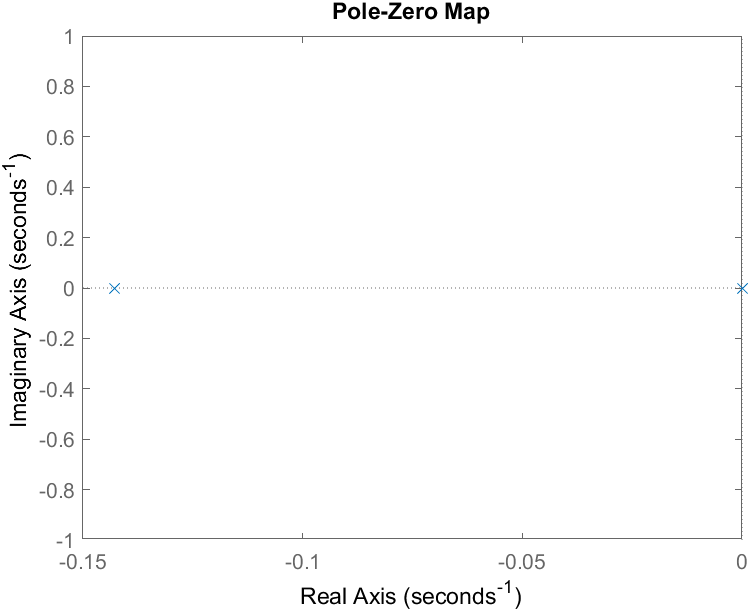
\includegraphics[width=0.8\textwidth]{{diagrams/pol_nullstellenplot.png}}
	\caption[Pol-Nullstellenplot]{Pol-Nullstellenplot}
	\label{fig:pnp}
\end{figure}